%versi 2 (8-10-2016) 
\chapter{Pendahuluan}
\label{chap:intro}

\section{Latar Belakang}
\label{sec:1:latar_belakang}
Ujian merupakan sebuah alat bantu untuk menilai pemahaman pelajar tentang ilmu yang diberikan oleh pengajar. Salah satu ujian yang diberikan kepada pelajar informatika adalah ujian koding yang biasanya dinilai berdasarkan ketepatan algoritma yang dipakai. Tetapi melakukan penilaian untuk setiap kode merupakan sebuah hal yang sulit untuk dilakukan karena dibutuhkannya waktu yang lama. Maka dari itu website \textit{judge} dibuat untuk memudahkan pekerjaan pengajar. 

\textit{Judge} merupakan sebuah website yang akan menilai sebuah kode dengan menjalankannya berdasarkan masukkan yang ditentukan dan menyamakan keluaran dari kode dengan keluaran yang sudah ditetapkan oleh pembuat soal dalam kurun waktu yang ditetapkan. Oleh karena itu, kode yang dibuat harus dapat mencakupi waktu yang diberikan dengan mengunakan algoritma yang tepat. Bukan hanya menilai dengan keluaran yang tetap tetapi \textit{judge} juga dapat mengunakan kode yang sudah dibuat oleh pengajar dan membandingkannya dengan keluaran kode yang di kumpulkan.

Sudah banyak perguruan tinggi informatika yang mengunakan website \textit{judge} dalam pemeriksaan kode pelajar termasuk perguruan UNPAR untuk penilai kode dari para mahasiswanya. Judge yang digunakan adalah SharIF-Judge~\cite{sharif} yang dimodifikasi oleh Stillmen Vallian terhadap Sharif-Judge~\cite{stillmen:sharif} buatan Mohammad Javad Naderi dengan \textit{framework} CodeIgniter dan Bash. Gambar~\ref{fig:dashboardpng} merupakan halaman utama setelah masuk ke dalam website SharIF-Judge.

\begin{figure}[H]
	\centering  
	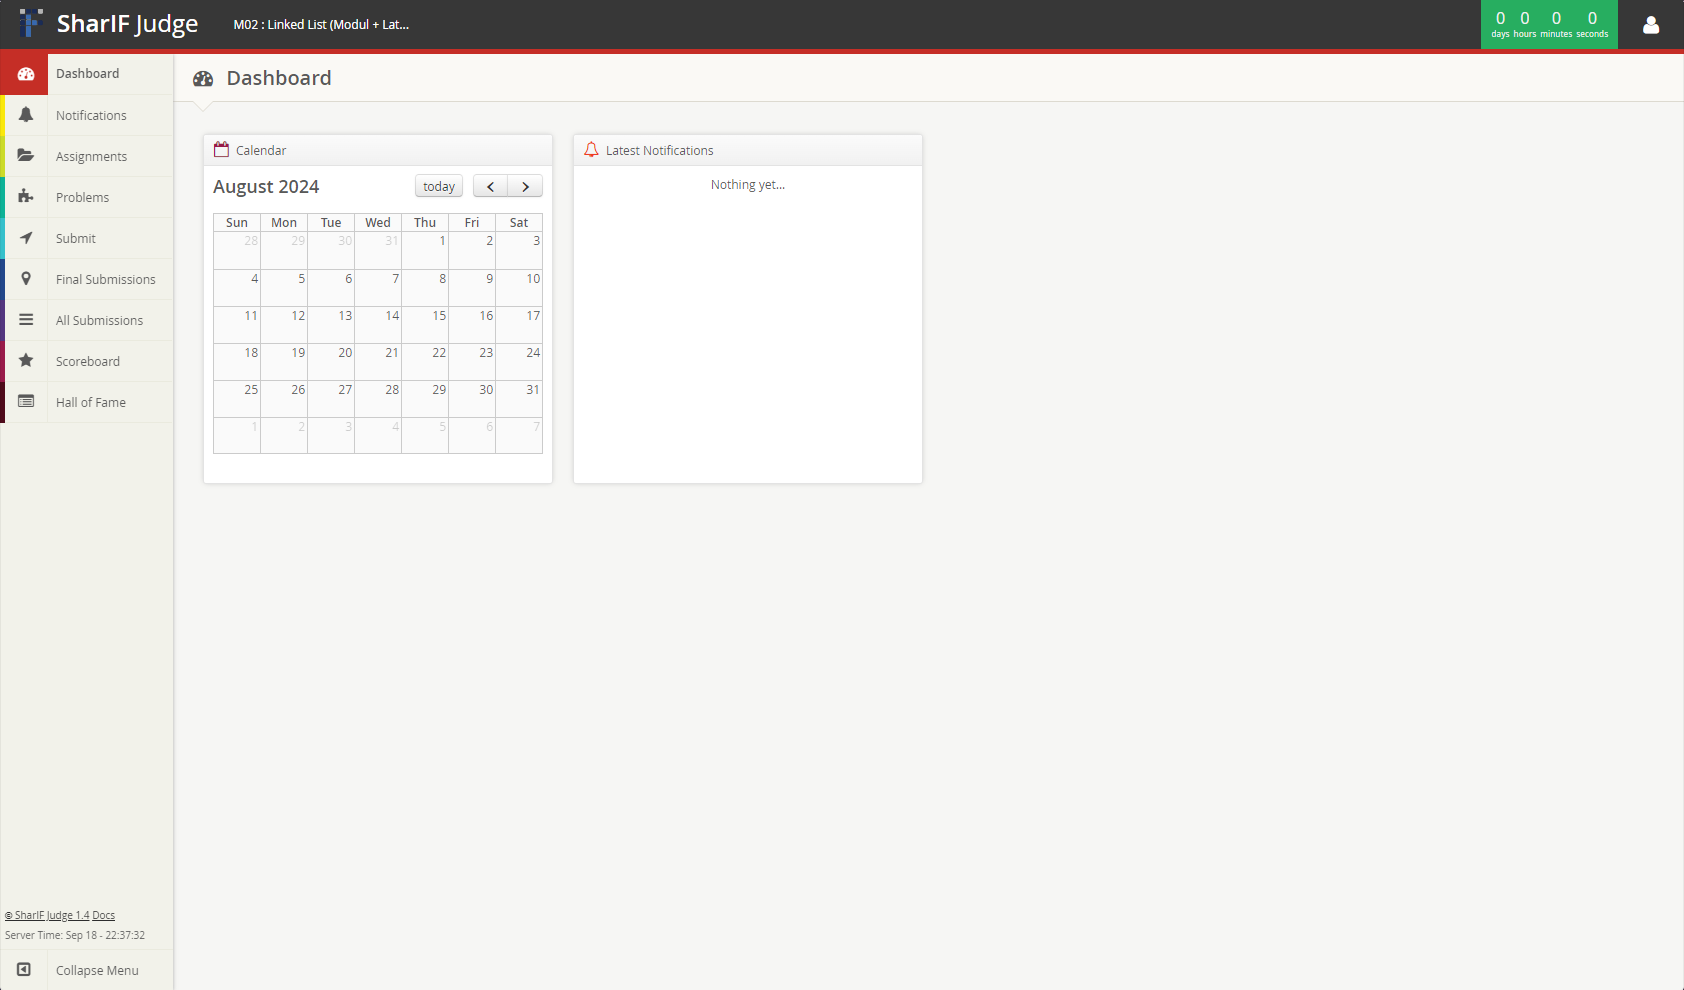
\includegraphics[scale=0.25]{dashboard}  
	\caption[Tampilan Awal SharIF Judge]{Tampilan Awal SharIF Judge} 
	\label{fig:dashboardpng} 
\end{figure} 

Tugas akhir ini merupakan sebuah pengembangan lanjutan dari tugas akhir yang bertopik "Implementasi editor kode pada Sharif Judge"~\cite{nicholas:sharif} oleh Nicholas Aditya Halim. Tugas akhir tersebut menceritakan bahwa SharIF-Judge tidak memiliki kemampuan untuk mengawasi proses pembuatan kode program karena para mahasiswa menggunakan aplikasi eksternal untuk pembuatan kode program tersebut. Sehingga dibuatnya modifikasi terhadap SharIF-Judge untuk menambahkan \textit{Intergrated Development Enviroment} (IDE), sebuah aplikasi untuk mengedit, mengompilasi, dan menjalankan kode program pada SharIF-Judge dengan editor kode bernama Ace~\cite{ace}. Gambar~\ref{fig:editor-kode} merupakan tampilan editor kode yang sudah diimplementasikan pada SharIF-Judge.

\begin{figure} 
	\centering  
	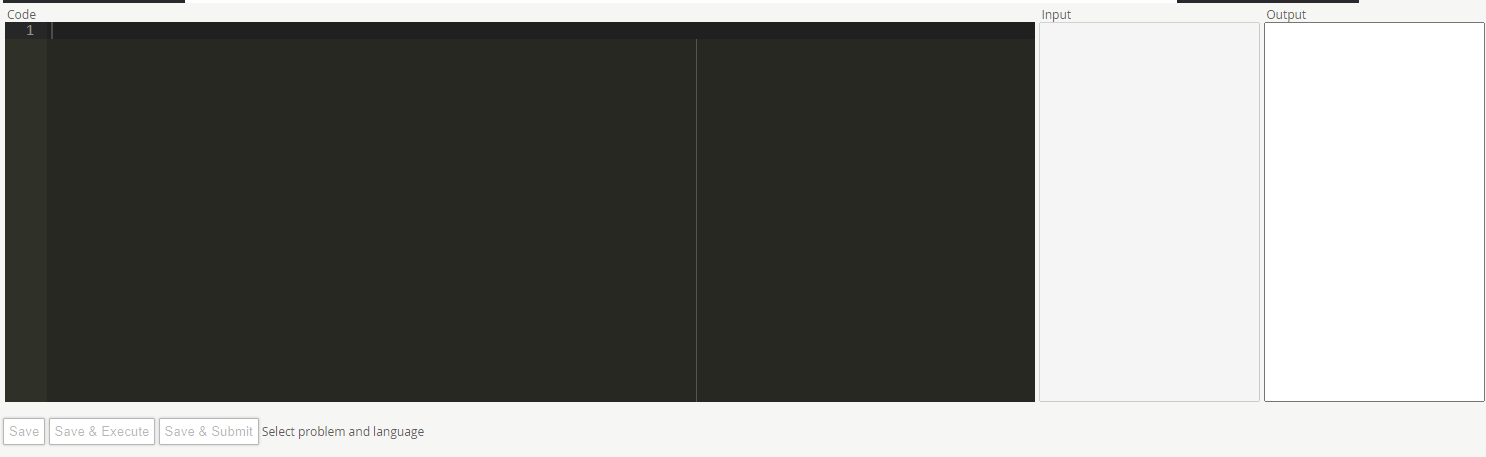
\includegraphics[scale=0.25]{kode-editor}  
	\caption[Tampilan editor kode pada SharIF-Judge]{Tampilan editor kode pada SharIF-Judge} 
	\label{fig:editor-kode} 
\end{figure} 

Pada tugas akhir ini, akan dibuat rekaman kode pada IDE yang tersedia di SharIF-Judge untuk membantu pengawasan dengan merekam dan memutar ulang ketikan mahasiswa. Tugas ini akan membuat pengawasan terhadap kegiatan kuliah lebih mudah untuk pengawas dan dapat menjadi bukti kecurangan jika dibutuhkan.

\section{Rumusan Masalah}
\label{sec:1:rumusan}

Rumusan Masalah yang akan dibahas pada tugas akhir ini adalah:
 \begin{enumerate}
     % \item Bagaimana agar editor kode lebih mudah untuk dipakai oleh mahasiswa.
     \item Bagaimana mengimplementasikan perekaman dan pemutaran ulang ketikan mahasiswa pada IDE SharIF-Judge?
     \item Bagaimana cara menyimpan data pemutaran ulang mahasiswa secara rutin dengan otomatis dan tidak mengambil penyimpanan \textit{database} sangat besar?
     \item Bagaimana tanggapan pengguna terhadap implementasi perekaman dan pemutaran ulang kode ketikan pada SharIF Judge?
 \end{enumerate}
 
\section{Tujuan}
\label{sec:1:tujuan}

Tujuan yang ingin dicapai skripsi ini adalah sebagai berikut:
    \begin{enumerate}
        \item Mengimplementasikan perekaman dan pemutaran ulang ketikan mahasiswa pada IDE SharIF-Judge.
        \item Mencari cara penyimpanan data efektif dan mengimplementasikannya pada perekaman dan pemutaran ulang ketikan. 
        \item Mendapatkan umpan balik dari tanggapan pengguna terhadap perekaman dan pemutaran ulang ketikan mahasiswa pada SharIF-Judge.
    \end{enumerate}
    
\section{Batasan Masalah}
\label{sec:1:batasan}

Pada pengerjaan tugas akhir ini terhadap batasan sebagai berikut:
    \begin{itemize}
        \item Perangkat lunak SharIF Judge hanya digunakan pada lingkungan Teknik Informatika Unpar.
        \item Perangkat lunak hanya dapat diuji pada mata kuliah pemrograman di mana dosen pembimbing terlibat.
    \end{itemize}

\section{Metodologi}
\label{sec:1:metlit}

Metodologi pengerjaan tugas akhir ini adalah sebagai berikut:
    \begin{enumerate}
        \item Melakukan studi mengenai komponen yang diperlukan untuk membuat sistem perekaman dan pemutaran ulang ketikan pada IDE berbasis web.
        \item Merancang sistem perekaman dan pemutaran ulang ketikan berbasis web untuk SharIF Judge
        \item Mengimplementasikan IDE berbasis web pada SharIF Judge.
        \item Melakukan pengujian dan eksperimen.
        \item Menulis dokumen tugas akhir.
    \end{enumerate}

\section{Sistematika Pembahasan}
\label{sec:1:sispem}

Sistematika pembahasan skripsi ini adalah sebagai berikut:
    \begin{itemize}
        \item Bab 1 Pendahuluan \\
        Membahas latar belakang, rumusan masalah, tujuan, batasan masalah, metodologi, dan sistematika pembahasan.
        \item Bab 2 Landasan Teori \\ 
        Membahas teori-teori yang berhubungan dengan penelitian ini, yaitu SharIF Judge, CodeIgniter 3, Twig, IDE, dan Ace.
        \item Bab 3 Analisis \\ 
        Membahas analisis terhadap perangkat lunak SharIF Judge dan IDE pada SharIF Judge.
        \item Bab 4 Perancangan \\ 
        Membahas perancangan fitur yang diimplementasikan pada SharIF Judge.
        \item Bab 5 Implementasi dan Pengujian \\ 
        Membahas implementasi fitur pada SharIF Judge dan pengjuan yang dilakukan.
        \item Bab 6 Kesimpulan dan Saran \\ 
        Membahas kesimpulan dari penelitian ini dan saran untuk penelitian berikutnya.
    \end{itemize}